\documentclass[a4paper,notitlepage]{article}
\usepackage{pfsstyle}
\title{Note on PFS humidity control \\ 
    (PFS SysEng study note PFS-SE-IPMU-00002-001+)}
\author{Atsushi Shimono}
\begin{document}
\renewcommand{\leftmark} {Note on PFS humidity control (PFS-SE-IPMU-00002-001+)}
\renewcommand{\rightmark}{Note on PFS humidity control (PFS-SE-IPMU-00002-001+)}

\maketitle
\tableofcontents

\section{Abstract}

This note is to have basic understandings on how we need to control humidity 
within our instrument. 


\section{Wator vapor calculation}

Using Wagner equation, saturated vapor pressure $P(T)$[kPa] is written as a 
formula of absolute temperature $T$[K]: 
\[ P(T) = P_{crit} \times \exp\left(\frac
     {A * (1-t) + B * (1-t)^{1.5} + C * (1-t)^3 + D * (1-t)^6}{1-t} \right) \]
\[ where \ : \  t = \frac{T}{T_{crit}} \]
with $P_{crit}, T_{crit}$ for critical point between gas and liquid. 
For water, 
$P_{cirt} = 22120 \text{[kPa]}, T_{crit} = 647.3 \text{[K]}$ 
and parapeters 
$A = -7.764510, B = 1.458380, C = -2.775800, D = -1.233030$
\footnote{These parameters are applicable between 275K to 647.14K, but 
similar below range.}, and values between -30 C and 20 C are drawn as 
Figure.~\ref{fig:sat-water-vapor}. 
Relative humidity is defined as the ratio of the partial pressure to the 
saturated vapor pressure. 

\begin{figure}[htb]
  \begin{center}
    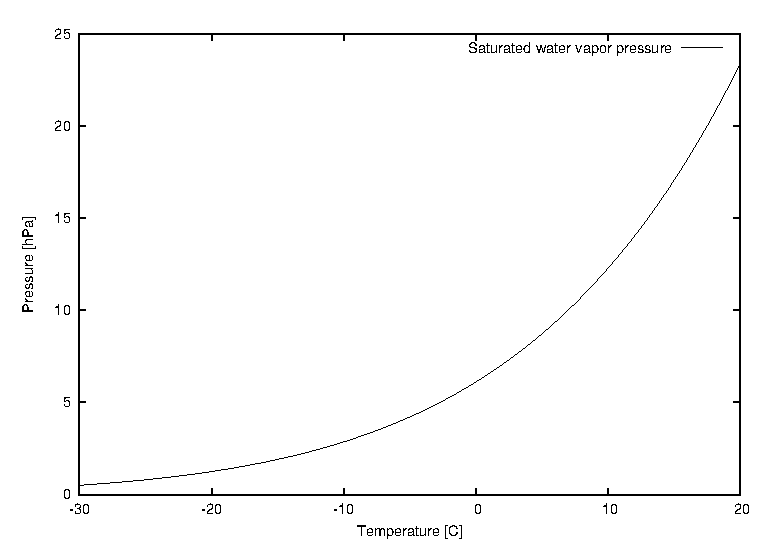
\includegraphics{PFS-SE-IPMU-00002-sat-pressure-water.eps}
  \end{center}
  \caption{Saturated water vapor pressure per temperature}
  \label{fig:sat-water-vapor}
\end{figure}

On the ideal gas law applicable, amount of the volumetirc (absolute) water 
vapor (in [g/m${}^3$]) 
changes on air temperature changed without any going in and out (since volume 
changes with temperature), and hard to examine on different temperatures. 
In this section, I will use (saturated) water vapor pressure for comparison. 
Figure.~\ref{fig:sat-humid-temp} shows graphs of relative humidities with the 
same water vapor pressure per temperature, which are maximum humidities 
not to condense on cooled surfaces 
\footnote{Note, this just considers water vapor and relative humidity, but not 
for surface conditions nor condensation nuclei.}. 
Also table.~\ref{tab:sat-humid-temp} shows relative humidities for 
various dew points. 

\begin{figure}[htb]
  \begin{center}
    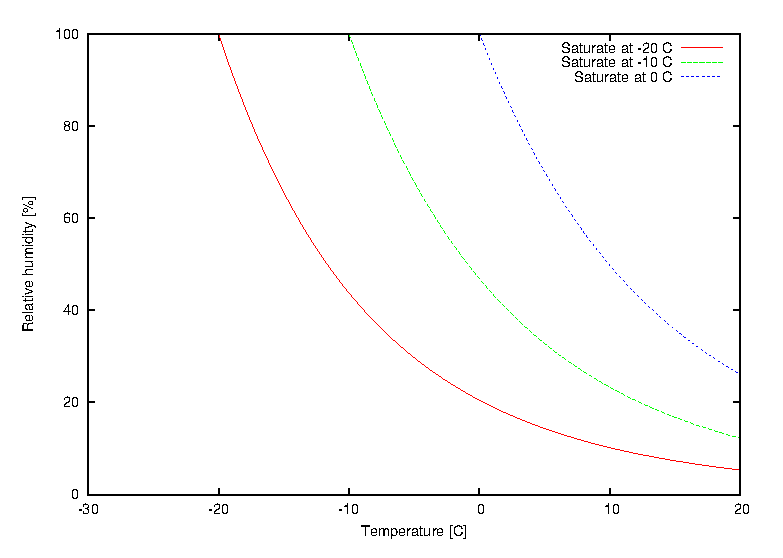
\includegraphics{PFS-SE-IPMU-00002-sat-humid-temp.eps}
  \end{center}
  \caption{Relative humidities with the same water vapor pressure}
  \label{fig:sat-humid-temp}
\end{figure}

\begin{table}[htb]
\begin{center}
\caption{Relative humidities for various dew points}
\label{tab:sat-humid-temp}
\begin{tabular}{c||r|r|r}
Dew point [C] & at 0 C & at 3 C & at 5C \\
\hline
  0 & 100.0 & 80.6 & 70.0 \\
- 5 &  69.0 & 55.6 & 48.3 \\
-10 &  46.8 & 37.8 & 32.8 \\
-15 &  31.3 & 25.2 & 21.9 \\
-20 &  20.5 & 16.5 & 14.4 \\
\end{tabular}
\end{center}
\end{table}



\section{Condition at PFS spectrograph}

In a document "Thermal Design and Performance IR (and VIS) Dewars" for SpS CDR 
2014 (March), CORRECTOR 1 has 278K at edge with 4K gradient. 
If the most cooled part in exposed to ambient is this corrector 1 and 
ambient is controlled at 3C, maximum relative humidity needs to be controlled 
under 75\%. 


\end{document}

